\chapter{Design methodology} \label{ch:designmet}
This chapter will describe a method for traversing between the algortihm domain and architecture domain in the A$^3$ model described in section \vref{sec:a3model} and the red lines in figure \vref{fig:a3method} shows where this movement occurs.\\

\begin{figure}[ht!]
  \centering
  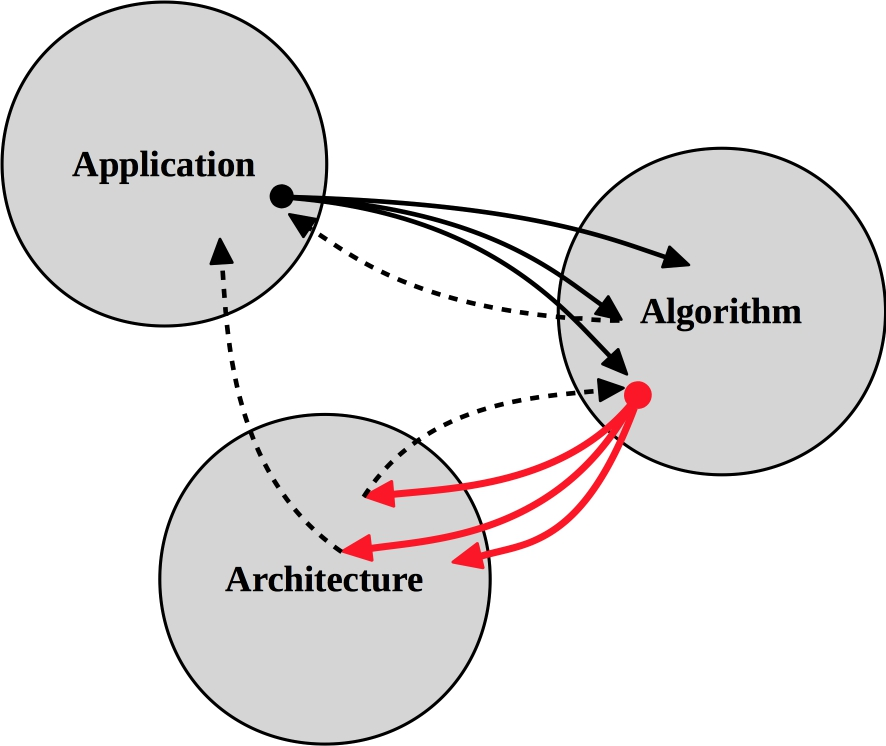
\includegraphics[scale=0.25]{figures/a3design}
  \caption{A$^3$ model with the movement from algorithm domain to architecture domain highlight}
  \label{fig:a3method}
\end{figure}

In \cite{gajski2009} the Gajski-Kuhn Y-chart is described and it is illustrated on figure \vref{fig:ychart_std}. This chart is a structured design method which can help organize the design processes for creating a dedicated hardware system. The chart consist of 3 domains: Behaviour, Structure, and Physical. The circles in the chart illustrates the different abstraction levels and following the arrows on the domain lines the abstraction levels increases.\\

\begin{figure}[ht!]
  \centering
  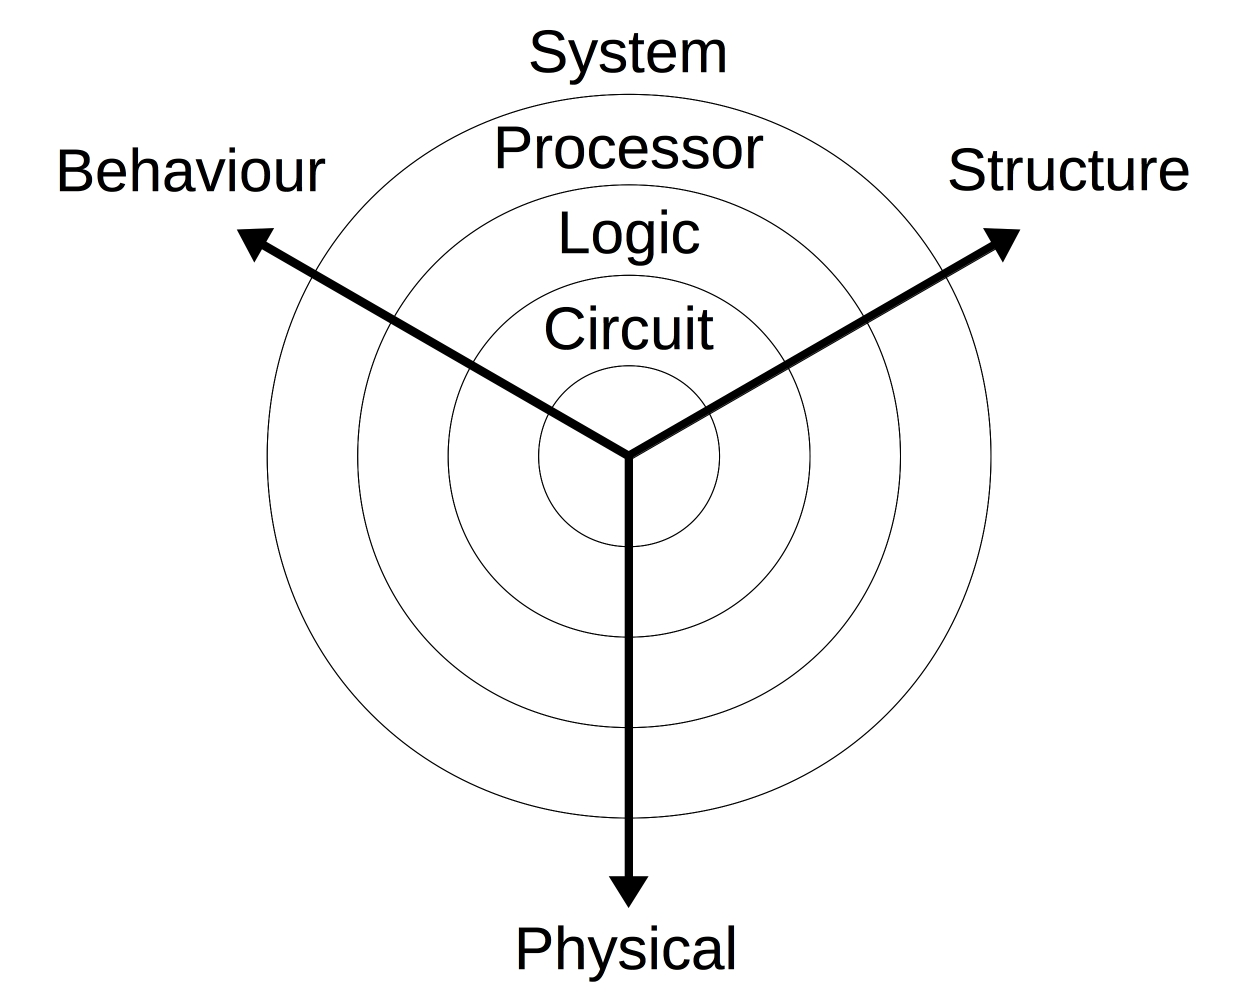
\includegraphics[width=0.475\textwidth]{figures/ychart-std.jpg}
  \caption{Illustration of the standard Gajski-Kuhn Y-chart \cite{gajski2009}\label{fig:ychart_std}}
\end{figure}

The behavioral domain describes the functional behavior of the system. Going from the highest abstraction level to the lower abstraction level this domain starts being described by algorithms and at the lowest level the behavior is described with differential equations.\\

The structural domain describes the system in terms of components and their interconnection. Going from the highest abstraction level to the lower abstraction levels this domain is first described using larger components such as platforms or CPUs and at the lowest level it will be described with transistors.\\

The physical domain describes how the system is physically put together and is at the highest abstraction levels described using chips, boards etc. and at lower levels, it will be described using transistor layout.\\

\begin{figure}[ht]
  \centering
  \begin{subfigure}[t]{0.475\textwidth}
    \centering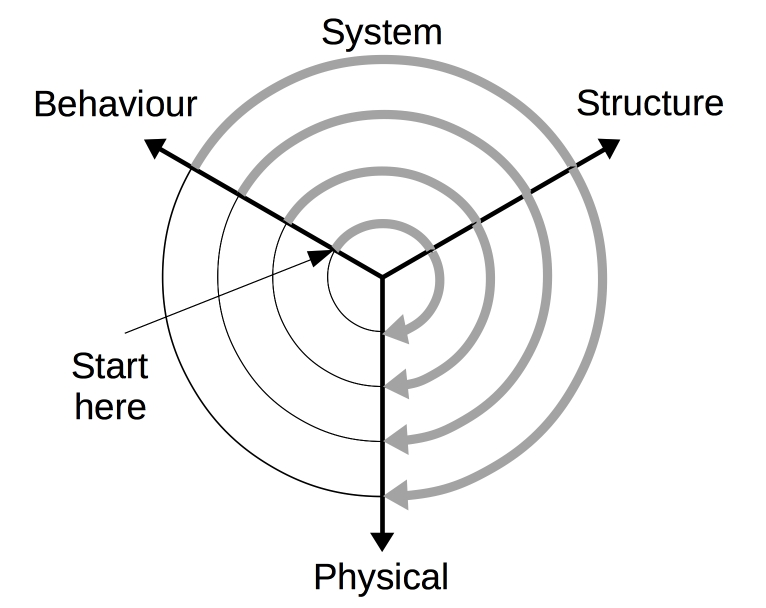
\includegraphics[width=\textwidth]{figures/bottom-up}
    \caption{Illustration of the Gajski-Kuhn Y-chart showing the bottom-up methodology \cite{gajski2009}  \label{fig:ybottom}}
  \end{subfigure}\hspace{0.5cm}
  \begin{subfigure}[t]{0.475\textwidth}
    \centering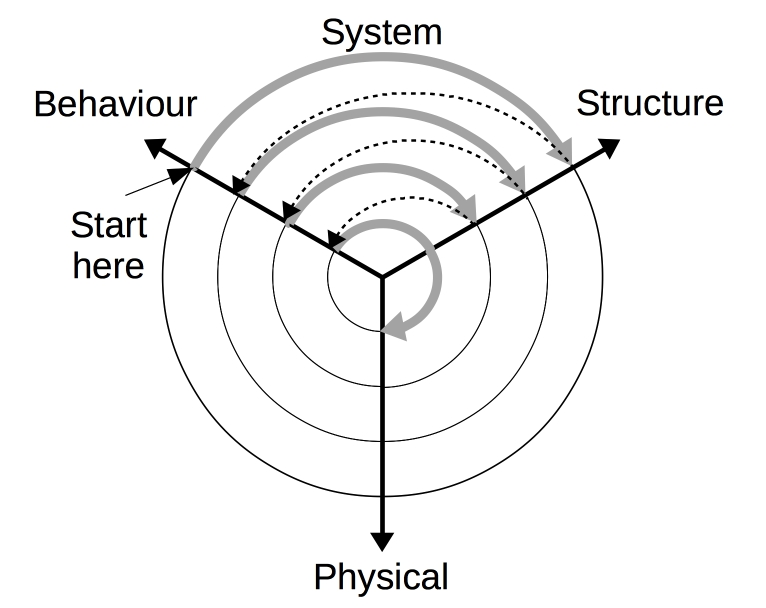
\includegraphics[width=\textwidth]{figures/top-down}
    \caption{Illustration of the Gajski-Kuhn Y-chart showing the bottom-up methodology \cite{gajski2009} \label{fig:ytop}}
  \end{subfigure}
  \caption{Illustration of different methodologies\label{fig:yboto}}
\end{figure}
Using the Y-chart for structuring the design process can guide the design process through different design methodology. Two basic methodologies are bottom-up and top-down. \\

The bottom-up methodology starts at the lowest abstraction level and moves through the 3 domains designing the system. Then it goes up a level and uses the results from the lower level to design next level. The bottom-up methodology gives full control of even the smallest details and the final cost function is available earlier. But designing at the lowest abstraction level can quickly be overwhelming and time-consuming due to all the details available at the lowest level. The bottom-up methodology is shown on figure \vref{fig:ybottom} \\

Top-down methodology instead starts at the highest abstraction level and designs the system going between the behavioral and structural domains and then go an abstraction level down and at the lowest level the system will be described in the physical domain. Since it starts at a higher abstraction level the design process is simpler and it is easier to optimize the system because amount of details to consider is less than at the lower abstraction levels i.e. it is easier designing a system connecting blocks/subsystems than it is connecting transistors. An issue with this methodology is that the exact cost function for the system is only available at the end of the design process when the design is finalized at the lowest abstraction level but is should be noticed that at higher abstraction levels an estimate of the cost function can be used. The top-down methodology is shown on figure \vref{fig:ytop}.\\

\begin{figure}[ht!]
  \centering
  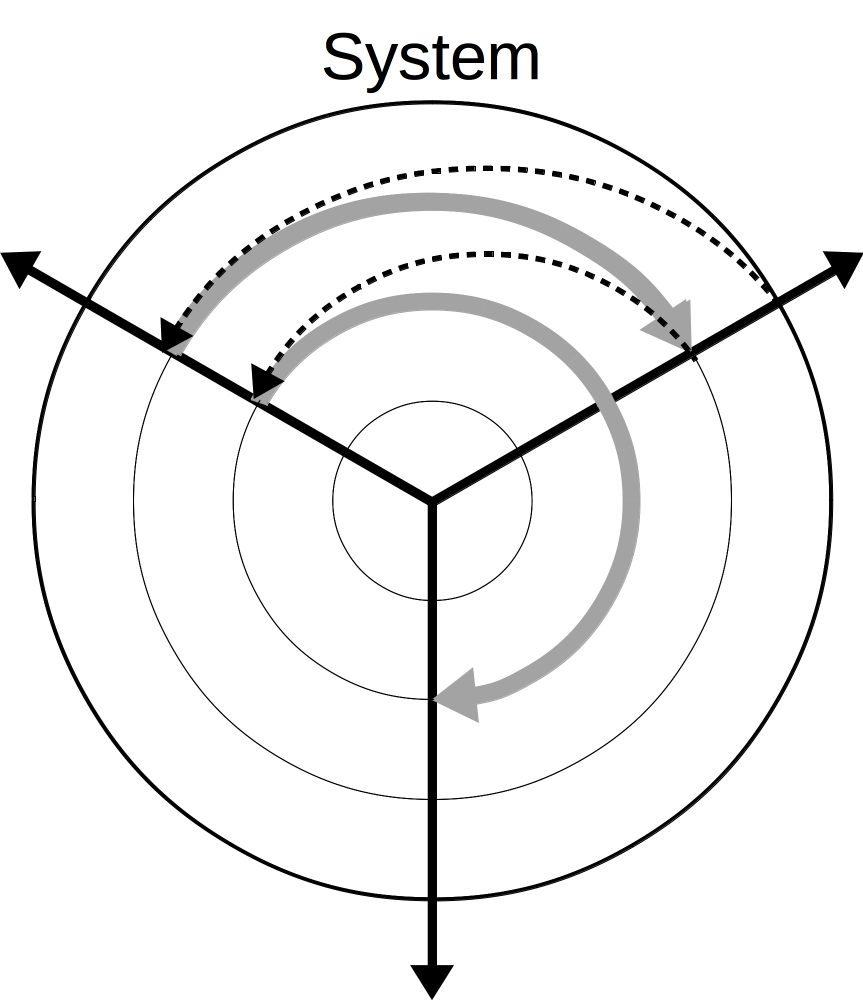
\includegraphics[width=0.475\textwidth]{figures/ychart-fpga.jpg}
  \caption{Illustration of the Gajski-Kuhn Y-chart showing the FPGA methodology \cite{gajski2009}  \label{fig:ychart_fpga}}
\end{figure}

Another methodology is the FPGA based methodology shown on figure \vref{fig:ychart_fpga} which is a variation of the top-down methodology. The methodology is based on the fabric of FPGA which consists of a large amount of Look-Up Tables (LUT). The top-down methodology is used at the system and processor abstraction levels where the processing and communication elements are expressed using LUTs. The design begins by mapping the application onto a platform and then custom components are expressed using LUTs. Once every component has been defined the whole design is flatten to LUTs and BRAMs and the tools provided by the FPGA supplier performs component placement and routing. This methodology have the same weaknesses as the normal top-down methodology and in addition to those weaknesses it is also unknown for the designer how the provided tools maps and connects the elements.\\

The Y-chart has been used for many years and therefore is well known but technology have evolved and the Y-chart have become less applicable in some cases. As discussed in chapter \ref{ch:plaanalysis} platforms for hardware and software co-design such as the Zynq platform have appeared. The Y-Chart is insufficient for these designs because the segregation of hardware and software is not naturally modeled on the chart. For these designs, new design models have been developed and one of these is the Rugby model \cite{jantsch1999rugby}. The model is not described in this project since it will not be used. As discussed in chapter \ref{ch:plaanalysis} this project will only focus on a FPGA design hence the GPP part of the Zynq platform is mostly ignored. Due to this the Y-chart and the FPGA methodology can and will be used for modeling the design for this project.

\section{Wrap-up}
The Y-chart and different design methodologies have been described and it is chosen to use the Y-chart and FPGA methodology to model the design for this project. If the GPP part of the Zynq were to be used in collaboration with the FPGA fabric another model such as the Rugby model should have been used but an FPGA implementation is the focus of this project and hence the Y-chart is used.

